\documentclass[preprint,12pt, a4paper]{elsarticle}

\usepackage{amsmath}
\usepackage{amssymb}
\usepackage{array}
\usepackage{booktabs}
\usepackage{color}
\usepackage{float}
\usepackage{graphicx}
\usepackage{ifpdf}
\usepackage[utf8]{inputenc}
\usepackage{keyval}
\usepackage{lineno}
\usepackage{listings}
\usepackage{longtable}
\usepackage{moresize}
\usepackage{multirow}
\usepackage{paralist}
\usepackage{rotating}
\usepackage{soul}
\usepackage{srcltx}
\usepackage{url}
\usepackage{xcolor}
\usepackage{xspace}
\usepackage{wrapfig}
\usepackage{subfig}
\usepackage{tikz}
\usepackage[export]{adjustbox} % http://ctan.org/pkg/adjustbox

\definecolor{listinggray}{gray}{0.95}
\definecolor{darkgray}{gray}{0.7}
\definecolor{commentgreen}{rgb}{0, 0.4, 0}
\definecolor{darkblue}{rgb}{0, 0, 0.6}
\definecolor{purple}{rgb}{0.6, 0, 0.6}
\definecolor{middleblue}{rgb}{0, 0, 0.75}
\definecolor{darkred}{rgb}{0.4, 0, 0}
\definecolor{brown}{rgb}{0.5, 0.5, 0}
\definecolor{dkgreen}{rgb}{0,0.5,0}
\definecolor{orange}{rgb}{1,.5,0}
\definecolor{dandelion}{cmyk}{0,0.29,0.84,0}

\usepackage[normalem]{ulem}
\makeatletter
\def\cyanuwave{\bgroup \markoverwith{\lower3.5\p@\hbox{\sixly \textcolor{cyan}{\char58}}}\ULon}
\def\reduwave{\bgroup \markoverwith{\lower3.5\p@\hbox{\sixly \textcolor{red}{\char58}}}\ULon}
\def\blueuwave{\bgroup \markoverwith{\lower3.5\p@\hbox{\sixly \textcolor{blue}{\char58}}}\ULon}
\font\sixly=lasy6 % does not re-load if already loaded, so no memory problem.
\makeatother

\def\BibTeX{{\rm B\kern-.05em{\sc i\kern-.025em b}\kern-.08em
    T\kern-.1667em\lower.7ex\hbox{E}\kern-.125emX}}

% Generate circled numbers
\newcommand*\circled[1]{\tikz[baseline=(char.base)]{
    \node[shape=circle,draw,inner sep=1pt] (char) {#1};}}
\newif\ifdraft{}
%\drafttrue{}

\ifdraft{}
  \newcommand{\amnote}[1]{ \textcolor{blue} { ***andrem: #1 }}
  \newcommand{\jhanote}[1]{ {\textcolor{red} { ***shantenu: #1 }}}
  \newcommand{\mtnote}[1]{ {\textcolor{orange} { ***matteo: #1 }}}
\else
  \newcommand{\amnote}[1]{}
  \newcommand{\jhanote}[1]{}
  \newcommand{\mtnote}[1]{}
\fi

\newcommand{\apples}{AppLeS\xspace}
\newcommand{\bj}{BigJob\xspace}
\newcommand{\computeunit}{Compute-Unit\xspace}
\newcommand{\computeunits}{Compute-Units\xspace}
\newcommand{\cloud}{cloud\xspace}
\newcommand{\clouds}{clouds\xspace}
\newcommand{\cc}{c\&c\xspace}
\newcommand{\CC}{C\&C\xspace}
\newcommand{\computedataservice}{Compute-Data Service\xspace}
\newcommand{\cu}{CU\xspace}
\newcommand{\cus}{CUs\xspace}
\newcommand{\dataunit}{Data-Unit\xspace}
\newcommand{\dataunits}{Data-Units\xspace}
\newcommand{\du}{DU\xspace}
\newcommand{\dus}{DUs\xspace}
\newcommand{\mrmg}{MR-Manager\xspace}
\newcommand{\MW}{master-worker\xspace}
\newcommand{\numrep}{8 }
\newcommand{\panda}{PanDA\xspace}
\newcommand{\pilot}{Pilot\xspace}
\newcommand{\pilots}{Pilots\xspace}
\newcommand{\pilotjob}{Pilot-Job\xspace}
\newcommand{\pilotjobs}{Pilot-Jobs\xspace}
\newcommand{\pilotcompute}{Pilot-Compute\xspace}
\newcommand{\pilotcomputes}{Pilot-Computes\xspace}
\newcommand{\pilotdata}{Pilot-Data\xspace}
\newcommand{\pilotdataservice}{Pilot-Data Service\xspace}
\newcommand{\pilotcomputeservice}{Pilot-Compute Service\xspace}
\newcommand{\prop}[1]{\textit{#1}\xspace}
\newcommand{\pilotmapreduce}{PilotMapReduce\xspace}
\newcommand{\pstar}{P*\xspace}
\newcommand{\pd}{PD\xspace}
\newcommand{\pj}{PJ\xspace}
\newcommand{\pjs}{PJs\xspace}
\newcommand{\pds}{Pilot Data Service\xspace}
\newcommand{\samplenum}{4 }
\newcommand{\su}{SU\xspace}
\newcommand{\sus}{SUs\xspace}
\newcommand{\schedulableunit}{Schedulable Unit\xspace}
\newcommand{\schedulableunits}{Schedulable Units\xspace}
\newcommand{\tmax}{\(T_{max}\)}
\newcommand{\tc}{\(T_{C}\)}
\newcommand{\tcnsp}{\(T_{C}\)}
\newcommand{\vocab}[1]{\textbf{#1}\xspace}

\newcommand{\B}[1]{\textbf{#1}\xspace}
\newcommand{\C}[1]{\textsc{#1}\xspace}
\newcommand{\F}[1]{\textbf{FIXME\@: #1}\xspace}
\newcommand{\I}[1]{\textit{#1}\xspace}
\newcommand{\T}[1]{\texttt{#1}\xspace}

\newcommand{\impterm}[1]{\texttt{#1}\xspace}

% System names
\newcommand{\bw}{\I{Blue\,Waters}}
\newcommand{\stampede}{\I{Stampede}}
\newcommand{\comet}{\I{Comet}}
\newcommand{\titan}{\I{Titan}}

% Latex Fu
\newcommand{\UPP}{\vspace*{-2.0em}}
\newcommand{\UP}{\vspace*{-1.0em}}
\newcommand{\up}{\vspace*{-0.5em}}

% Paper specific Macro's
\newcommand{\ru}{$RU$\xspace}
\newcommand{\ttc}{$ttc$}
\newcommand{\ttca}{$ttc_a$}

% Table multirows
\newcommand{\mr}[1]{\multirow{2}{*}{#1}}%
\newcommand{\mc}[2]{\multicolumn{#1}{l}{#2}}

\lstdefinestyle{myListing}{
  frame=single,   
  backgroundcolor=\color{listinggray},  
  %float=t,
  language=C,       
  basicstyle=\ttfamily \footnotesize,
  breakautoindent=true,
  breaklines=true
  tabsize=2,
  captionpos=b,  
  aboveskip=0em,
  belowskip=-2em,
}      

\lstdefinestyle{myPythonListing}{
  frame=single,   
  backgroundcolor=\color{listinggray},  
  %float=t,
  language=Python,       
  basicstyle=\ttfamily \footnotesize,
  breakautoindent=true,
  breaklines=true
  tabsize=2,
  captionpos=b,  
}

% This is now the recommended way for checking for PDFLaTeX:
\ifpdf{}
  \DeclareGraphicsExtensions{.pdf, .jpg, .tif}
\else
  \DeclareGraphicsExtensions{.eps, .jpg, .ps}
\fi

\tolerance=1000
\hyphenpenalty=10


\journal{SoftwareX}

\begin{document}
\begin{frontmatter}

\title{RADICAL-Cybertools: Middleware Building Blocks for Scalable Science}

\author{Aymen Al Saadi$^1$, Shantenu Jha$^{1,2}$, Andre Merzky$^1$, Mikhail Titov$^2$ and Matteo Turilli$^{1,2}$}
\address{$^1$Electrical \& Computer Engineering, Rutgers University, Piscataway, NJ 08854, USA, $^2$Brookhaven National Laboratory}

\begin{abstract}
% Ca. 100 words
RADICAL-Cybertools (RCT) are middlware software systems to develop efficient and
effective tools for scientific computing. Specifically, RCT enable developing
applications with up to 100,000 heterogeneous tasks and execute them on the
largest high performance computing platforms in the world. RCT are building
blocks designed to work as stand-alone systems, integrated among themselves or
with third-party systems. RCT enable innovative science in multiple domains,
including biophysics, climate science, particle physics and drug discovery,
consuming hundreds of millions of core hours/year. This paper provides an
overview of RCT, their impact, and their underlying software engineering and
architectural principles.
\end{abstract}

\begin{keyword}

%% keywords here, in the form: keyword \sep keyword
Middleware \sep Pilot System \sep Building Blocks

%% PACS codes here, in the form: \PACS code \sep code

%% MSC codes here, in the form: \MSC code \sep code
%% or \MSC[2008] code \sep code (2000 is the default)

\end{keyword}

\end{frontmatter}

% \linenumbers{}

% {\em The manuscript must be submitted in single column. The following
% constraints apply:
% \begin{enumerate}
%   \item Word count: max. 3000. Excluding: title, authors, affiliations,
%         references, metadata tables; Including: abstract, running text,
%         captions, footnotes.
%   \item Max. 6 figures.
%   \item The manuscript must have line numbers.
%   \item At least one of the two mandatory metadata tables located at the
%         end of the article template must be filled in and included in the
%         manuscript.
%   \item To submit your code/software you can: Point to an external location
%         (repository, archive, etc.) where the code is publicly available.
%         Clearly mark the address to retrieve the code in the metadata
%         tables included in the manuscript.
% \end{enumerate}}


% ---------------------------------------------------------------------------
% Section I
% ---------------------------------------------------------------------------
\section{Motivation and significance}\label{sec:motivation}

% {\em Guidelines for the authors:
% \begin{enumerate}
%   \item Introduce the scientific background and the motivation for
%         developing the software.
%   \item Explain why the software is important, and describe the exact
%         (scientific) problem(s) it solves.
%   \item Indicate in what way the software has contributed (or how it will
%         contribute in the future) to the process of scientific discovery;
%         if available, this is to be supported by citing a research paper
%         using the software.
%   \item Provide a description of the experimental setting (how does the
%         user use the software?).
%   \item Introduce related work in literature (cite or list algorithms used,
%           other software etc.).
% \end{enumerate}}

The design of middleware to support scientific computing has never been more
challenging. The unprecedented complexity of middleware design and development
arises from diversity in application requirements, disruptive changes in the
resources and technology landscapes, intermixed with new discovery modalities
and need for scalable computing. Against this dynamic landscape, two critical
challenges must be addressed: (1) How can middleware be designed and implemented
to meet the collective challenges of scale, new and diverse functionality, and
usability? (2) How can critical middleware components be designed to be
sustainable software implementations while being forward-looking and enable
innovative capabilities?

RADICAL-Cybertools (RCT)~\cite{github-rct} are a set of systems developed to
address those challenges.  RCT are building blocks, which can be used as a
stand-alone system, or integrated with other RCT, or third-party tools to enable
diverse functionalities.
% RCT offer several innovative features to support the design and implementation
% of middleware.
This paper takes a software perspective to present the architectural paradigm of
RCT and discuss the design and implementation of
% two cybertools:
RADICAL-Pilot and RADICAL-EnsembleToolkit (EnTK). We outline the direct impact
that RCT are having on domain sciences, focusing the discussion on architectural
and design paradigms of middleware for scientific computing. In this way, we
show how RCT further
% the ``state-of-theory'' and practice of
scientific computing.


% ---------------------------------------------------------------------------
% Section II
% ---------------------------------------------------------------------------
\section{Software description}\label{sec:description}

% {\em Describe the software in as much as is necessary to establish a
% vocabulary needed to explain its impact.}

% \vbnote{the abbreviation RCT is being overwritten here, already defined RCT
% in Section 1}

RCT have three main components: RADICAL-SAGA (RS)~\cite{merzky2015saga},
RADICAL-Pilot (RP)~\cite{merzky2018using} and RADICAL-EnsembleToolkit
(EnTK)~\cite{balasubramanian2016ensemble,balasubramanian2018harnessing}.
RS is a Python implementation of the Open Grid Forum SAGA standard
GFD.90~\cite{goodale2006saga},
% a high-level interface to distributed infrastructure components like job
% schedulers, file transfer and resource provisioning services. RS
which enables interoperability across high performance computing (HPC)
platforms.
% heterogeneous distributed infrastructures, improving on their usability and
% enhancing the sustainability of services and tools.
Ref.~\cite{merzky2015saga} details RS, therefore we focus on RP and EnTK in the
rest of the paper.

RP is a Python implementation of the pilot paradigm and architectural
pattern~\cite{turilli2018comprehensive}. Pilot systems enable users to submit
jobs to HPC platforms and then use the resources acquired to execute the
application tasks. These tasks are directly scheduled via the pilot system,
without having to queue in the platform's batch system.

EnTK is a Python implementation of a workflow engine, specialized in supporting
the programming and execution of applications with ensembles of tasks organized
into pipelines of stages of tasks. EnTK executes tasks concurrently or
sequentially, depending on their priority relation and resource availability.

Distinctively, RCT supports heterogeneous executable or function tasks. Both
types of task can be single/multi core/GPU/node and MPI/OpenMP\@. Executable
tasks are programs that run as self-contained entities, while function tasks are
functions or methods written in a specific programming language. Uniquely, RCT
support the concurrent execution of heterogeneous executable and Python function
tasks across up to 500,000 cores and 36,000 GPUs.
% acquired on among the largest HPC platforms currently available to the
% scientific research.

% Both RP and EnTK focuses on High Performance Computing (HPC) resources,
% enabling the concurrent and consecutive execution on CPU/GPU of stasks.

% RP focuses on High Performance Computing (HPC) resources, enabling the
% concurrent and consecutive execution of heterogeneous workloads comprised
% of one or more scalar, MPI, OpenMP, multi-process, and multi-threaded
% tasks. These tasks can be executed on CPUs, GPUs and other accelerators, on
% the same pilot or across multiple pilots.

% EnTK promotes ensembles of tasks to a high-level abstraction, providing a
% programming interface and execution model specific to ensemble-based
% applications. EnTK is engineered for scale and a diversity of computing
% platforms and runtime systems, agnostic of the size, type and coupling of
% the tasks comprising the ensemble.

RCT work both individually and as an integrated system, with or without third
party software systems. This requires a ``Building Block'' approach to their
design and development, based on applying the traditional notions of modularity
at system level~\cite{turilli2019middleware}. The Building Block approach
derives from the work on Service-oriented Architecture and its Microservice
variants, and the component-based software development approaches where
computational and compositional elements are explicitly
separated~\cite{garlan1995architectural,clemens1998component,schneider2000components}.

% batory1992design, lenz1987software,}. \jhanote{Can we reduce the number of
% references to SOA and CBSE? I'm assuming some of these are in the CCGrid and
% CISE paper, so "references therein" is acceptable. It is motivated as much by
% space, as it consistency across other "aspects" not central to this paper or
% covered elsewhere.}

% \jhanote{ We should not say the  later part, as I don't think its fully
% correct.} % AirFlow, Oozie, Azkaban, Spark Streaming, Storm, or Kafka are
% examples of tools that have a design consistent with the building blocks
% approach.

% In our adaptation, the Building Block approach is based on four
% well-understood principles: self-sufficiency, interoperability, composability,
% and extensibility. This approach does not reinvent modularity, it applies it
% at system level to enable composability among independent software systems. As
% an abstraction, modularity enables separation of concerns by encapsulating
% discrete functions into semantic units exposed by means of a dedicated
% interface. As such, modularity can be used at function or method level,
% depending on the programming paradigm and the facilities offered by
% programming languages, or at system-level, depending on the interface exposed
% by each system.

% ---------------------------------------------------------------------------
\subsection{Software Architecture}\label{ssec:architecture}

% {\em Give a short overview of the overall software architecture; provide a
% pictorial component overview or similar (if possible). If necessary provide
% implementation details.}

Architecturally, all RCT consist of one or more subsystems, each with several
components. Some components are used only in specific deployment scenarios,
depending on both application requirements and resource capabilities. Some
components can be instantiated concurrently, enabling throughput scaling. A
communication overlay enables coordination of concurrent components, improving
scalability at the cost of infrastructure-specific overheads.

% \vbnote{I think mesh refers to a topology where every component can directly
% talk to another. I don't think that's true for our systems - I think we have a
% master-slave comm. model.}\mtnote{The communication mash is among components
% of subsystems, e.g., RP agent's components, or workflow manager in
% entk.}\jhanote{I've added to the confusion by using overlay. I think mesh is
% usually used in topology specific context, and that is not intended. I wanted
% to use communication subsystem -- which is the canonical approach, but we're
% talking about subsystems of components, thus subsystem is suboptimal.}

% Concurrent components are coordinated via a dedicated A  communication mesh,
% which introduces runtime and infrastructure-specific overheads, but improves
% overall scalability of the system and lowers component complexity. Components
% can have different implementations; configuration files can tailor each RCT to
% specific resources types, workloads, or scaling requirements. Components
% exchange data about the entities specific to each RCT and data about the state
% of the components and subsystems. Each type of data has dedicated modules and
% communication channel, separating communication from coordination with
% explicit states and events for each entity.

% Ref.~\cite{merzky2015saga} details RADICAL-SAGA architecture and capabilities.
% In the rest of the paper, we focus on RP and EnTK, first introducing each
% system individually, then showing how RCT as a whole can be composed to serve
% diverse use cases.

% ------------
\subsubsection{RADICAL-Pilot}\label{sssec:arch_rp}

RP implements two abstractions: Pilot and Task. Pilots are placeholders for
computing resources, where resources are represented independent of
architecture and platform details. Tasks are units of work specified by a
program's executable or a language-specific function/method, alongside resource
and execution environment requirements.

Fig.~\ref{fig:archs}a depicts RP's architecture with two subsystems (white
boxes), each with several components (purple and yellow boxes). Purple
components manage pilots and tasks while yellow components enable communication
and coordination. Subsystems can execute locally or remotely, communicating over
TCP/IP and enabling multiple deployment scenarios.
% For example, users can run Client locally, and distribute MongoDB and one
% or more instances of Agent on remote computing infrastructures.
% Alternatively, users can run all components on a local or remote resource.

% \vbnote{Is 'AgentManager' a communication sub-component? Also, in the
% figure Queues are either blue or orange but in the legend they are blue and
% pink.}

\begin{figure}
    \centering
    \subfloat[ ]{{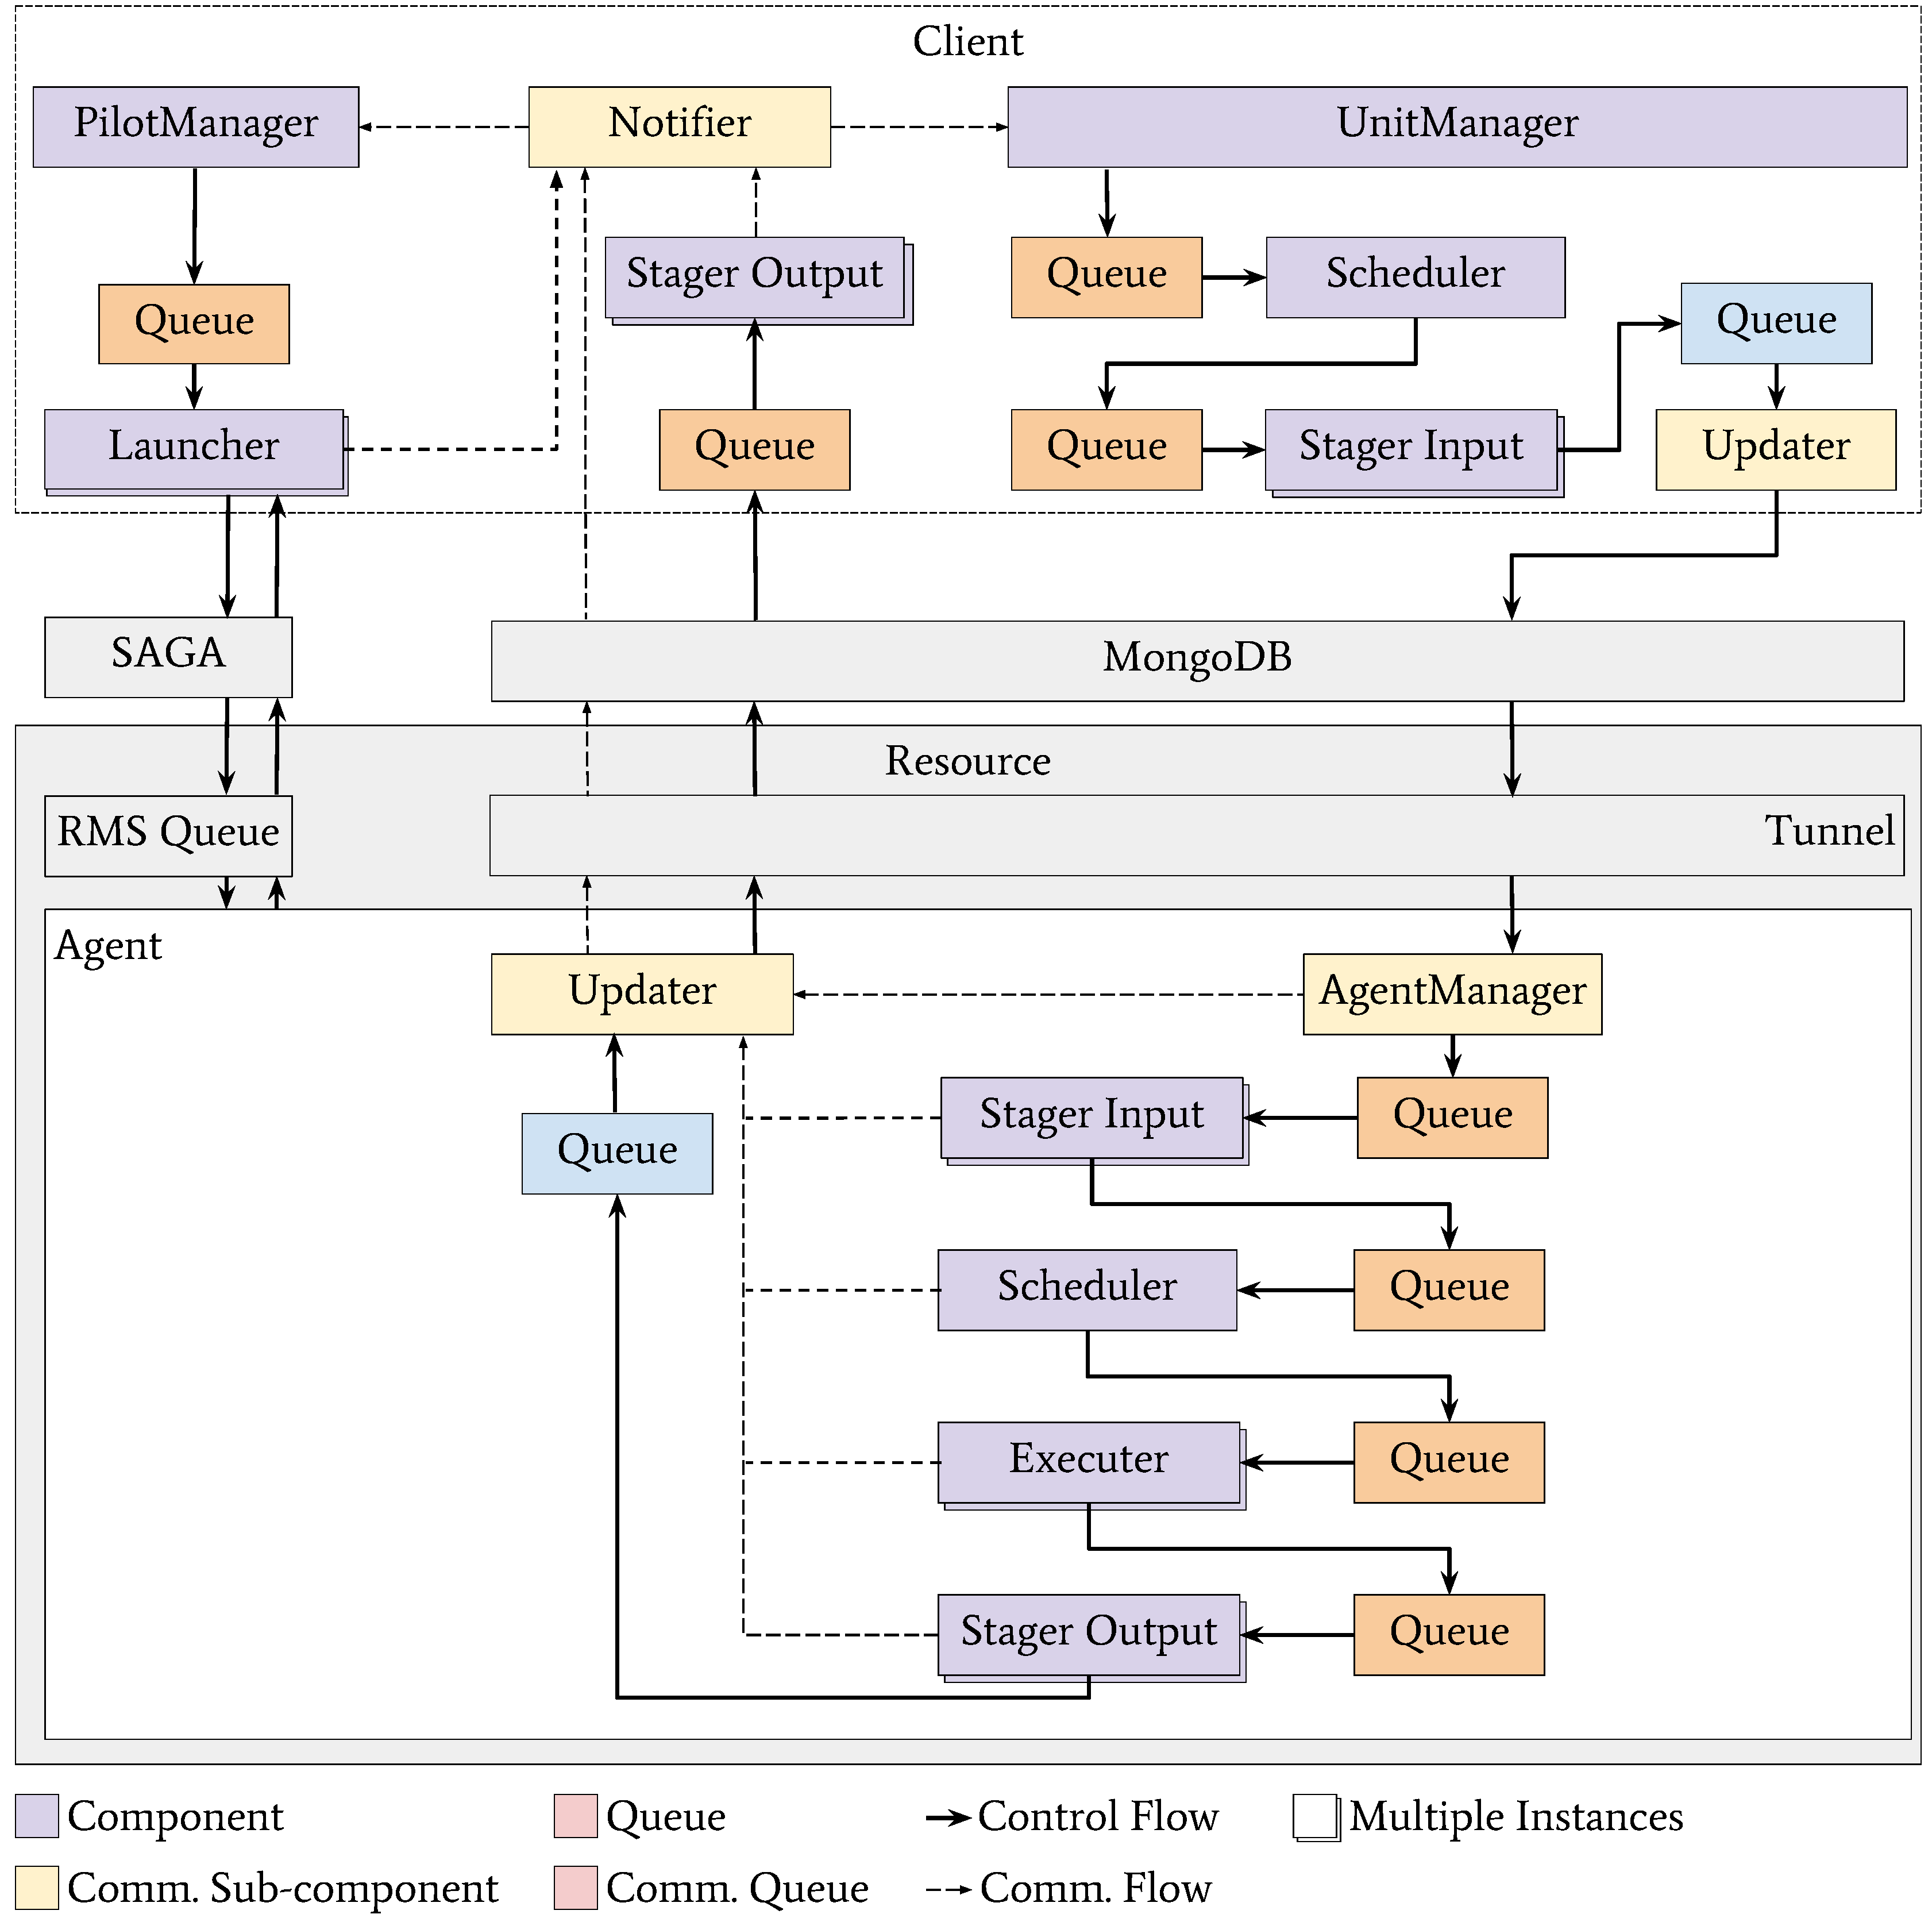
\includegraphics[width=0.555\textwidth]{figures/arch_rp.pdf} }}
    \qquad
    \subfloat[ ]{{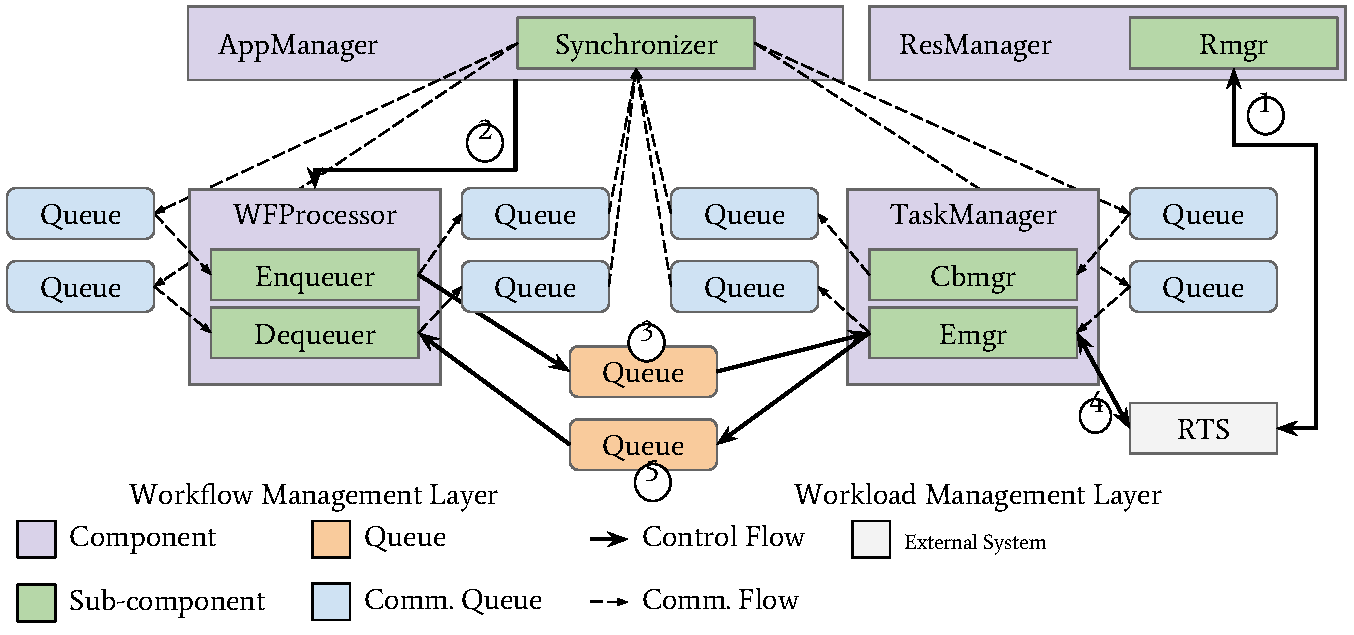
\includegraphics[width=0.34\textwidth]{figures/arch_entk.pdf}
    }} \caption{Caption. \mtnote{TODO\@: Fix EnTK AppManager; replace unit with
    task}}\label{fig:archs}
\end{figure}

% Client has two main components: PilotManager and UnitManager. PilotManager
% manages pilots and has a main component called `Launcher'. Launcher uses
% resource configuration files to define the number, placement, and
% properties of the Agent's components of each pilot. Currently,
% configuration files are made available for all the HPC machines of the
% Extreme Science and Engineering Discovery Environment (XSEDE), Blue Waters
% at the National Center For supercomputing Applications (NCSA), Cheyenne at
% NCAR-Wyoming Supercomputing Center (NWSC), and Rhea, Titan and Summit at
% the Oak Ridge National Laboratory (ORNL). Users can provide new files or
% alter existing configuration parameters at runtime, both for a single pilot
% or a whole RP session.

% UnitManager manages CUs and has two main components: Scheduler and
% StagerInput. Scheduler schedules CUs onto one or more pilots, available on
% one or more machines. This enables late binding of CUs to resources,
% depending on their availability. CUs are bound to resources that satisfy
% their execution requirements only when these resources are actually
% available. StagerInput distributes the input files that CU may need for
% their execution to the machines on which each CU has been scheduled.

RP's Client has two main components: PilotManager and TaskManager. PilotManager
manages pilots, using the Launcher and its configuration files to tailor RP's
Agent to specific platforms. Currently, RP supports 17
platforms~\cite{rp-supported-url} across DoE laboratories, NSF ACCESS and
university campuses. The TaskManager manages tasks, using the Scheduler to bind
and launch tasks onto one or more pilots, across one or more platforms. The
StagerInput copies tasks' input files to the machine on which each task was
scheduled.

% Agent and has four components: StagerInput and StagerOutput for staging
% CUs' input and output data, Scheduler and Executer to schedule CUs on a
% pilot resources and execute those CUs on them. Multiple instances of the
% Stager and Executer components can coexist in a single Agent. Depending on
% the architecture of the target machine, Agent's components can individually
% be placed on cluster head nodes, MOM/batch nodes, compute nodes, virtual
% machines, or any combination thereof. ZeroMQ communication bridges connect
% the Agent components, creating a network to support the transitions of CUs
% through components.

RP's Agent has four main components: StagerInput and StagerOutput for staging
task's input/output data, Scheduler and Executer to schedule and execute tasks
on the pilot(s) resources. For performance at scale, multiple instances of the
Stager and Executer can coexist in multiple sub-agents, placed on MOM/batch
nodes, compute nodes, virtual machines, depending on the architecture of each
platform.

% Each component of each subsystem of RP has a dedicated queue to feed
% entities into that component. Orange Queues in Fig.~\ref{fig:archs}a are
% dedicated to pilots and CUs, blue Queues to the messages exchanged by
% communication components. All Queues support bulk communication to obtain
% performance at scale in a distributed systems. Further, queues enable load
% balancing among concurrent components. Note that concurrent components are
% used for performance optimization at scale.

Each Agent component has a queue to support the exchange of pilot or task
descriptions (Fig.~\ref{fig:archs}a, orange queues), and of control messaging
(Fig.~\ref{fig:archs}a, blue queues). All queues support bulk communication and
enable load balancing among concurrent components to obtain performance at
scale.
%
% Data management in RP focuses on providing input files to CUs before their
% execution, and on moving output files to later CUs, or back into the user
% environment. On HPC resources which provide both local and network storage,
% RP can select the most appropriate storage, depending on CUs I/O
% requirements.  Data can be exclusive to CUs, or can be shared between CUs.
%
RP moves, copies or links input files to tasks before execution and output files
from tasks after execution. RP can select the most appropriate storage location,
depending on resource capabilities and task requirements. Data can be exclusive
to each task, or shared among tasks.
%
% A special queue instance is rendered as collection in a MongoDB database.
% That collection is used to communicate between Client and Agent, while
% preserving the semantics used for all other queues in
% Fig.~\ref{fig:archs}a. Since the MongoDB entries are persistent, that
% database is also used to store data for \textit{post mortem} profiling and
% analysis.
%
RP's Client and Agent communicate via a queue instance rendered as a data
structure of a database, preserving the semantic of the queues in
Fig.~\ref{fig:archs}a. Database's data are persistent, contributing to
\textit{post mortem} profiling and analysis of RP executions via
RADICAL-Analytics~\cite{radical-analytics}.

Fig.~\ref{fig:archs}a's numbers show the resource acquisition and task execution
process. The PilotManager uses RADICAL-SAGA to queue a pilot as a job on an HPC
platform's batch system (Fig.~\ref{fig:archs}a.1--2). Once scheduled, the job
bootstraps RP's Agent and the Agent's Updater notifies RP's Client that tasks
can be executed (Fig.~\ref{fig:archs}a.3). Upon notification, the client's
TaskManager queues all the available tasks onto the client's Scheduler and,
after staging files when required, tasks are queued to the agent's Scheduler
(Fig.~\ref{fig:archs}a.4-6). The agent's scheduler assigns tasks to suitable
portions of the available pilot's resources and then queues those tasks to an
Executor (Fig.~\ref{fig:archs}a.7). The agent's Executor places each task on the
assigned resources, sets up their execution environment, and then launches each
task for execution (Fig.~\ref{fig:archs}a.8).


% ------------
\subsubsection{RADICAL Ensemble Toolkit}\label{sssec:arch_entk}

EnTK implements three abstractions: Task, Stage and Pipeline. EnTK and RP share
the same Task abstraction but, in EnTK, a Stage is a set of tasks which have no
mutual dependencies and thus can execute concurrently; and a Pipeline is a
sequence of stages where the ordering of the stages represents the ordering of
their execution.

% As with RP, EnTK enables concurrent and sequential execution of set of
% executable or function tasks. Each task's program can use parallelism,
% enabling concurrent execution of scalar, MPI, OpenMP, multi-process, and
% multi-threaded programs.

Fig.~\ref{fig:archs}b shows the architecture of EnTK (white) with three
components (purple), each with subcomponents dedicated to the management of
EnTK's entities (green) or coordination of the entities' execution (yellow). The
three components are AppManager, WFProcessor and TaskManager, respectively
enabling workflow specification, and workflow and task management. EnTK is a
workflow engine and, as such, it leverages a third-party runtime system (RTS)
for task execution.

% \amnote{I would probably leave out the "RabbitMQ" box and label - that the
% queues are implemented in RMQ is an implementation detail, similar to ZMQ
% on RP?  It's also (rightly) not mentioned in the
% text.}\mtnote{Done.}\amnote{nitpicking mode (meaning: feel free to ignore,
% its inconsequential in this paper): we don't mention a "QueueManager"
% either. Is that really a notable EnTK component?  I would suggest to leave
% out the whole grey box as being not an architectural element, but an
% implementation detail. The has a wierd shape anyway, which I think is owed
% to unclarity in it's role?}

EnTK's API enables the development of ensemble-based applications
% with tasks, stages and pipelines,
and the specification of resource requirements for the application execution.
AppManager initializes EnTK and holds the global state of the application at
runtime. AppManager is the sole stateful component of EnTK, allowing to restart
other components upon failure, without interrupting the execution of the
ensemble-based application.

WFProcessor queues and dequeues tasks pulled to and from the TaskManager in
accordance with the task order specified by stages and pipelines. TaskManager
interfaces with the RTS via ResManager and ExecManager. RTS provides
capabilities to acquire resources and schedule tasks on those resources for
execution. ResManager isolates RTS from EnTK, enabling fault-tolerance with
persistent information about executed tasks. ExecManager schedules tasks on
the resources, tracking the state of each task during execution. Currently,
EnTK support only RP as RTS but it is designed to use other task-based RTS
as, for example, Coasters or HTCondor.

Fig.~\ref{fig:archs}b's numbers illustrate the execution of workflows in
EnTK\@. Users instantiate an AppManager, %(Lis.~\ref{code:amgr}),
define a set of resources on which to run their workflow,
% (Lis.~\ref{code:res}),
describe that workflow in terms of pipelines, stages and tasks
% (Lis.~\ref{code:pst})
and execute it.
% (Lis.~\ref{code:exec}).
AppManager passes a copy of the workflow description to WFProcessor that, based
on the priorities between stages and pipelines, uses Enqueuer to queue tasks
that are ready for execution to TaskManager (Fig.~\ref{fig:archs}b.1).
Meanwhile, ResManager users the chosen runtime system to acquire the requested
resources (Fig.~\ref{fig:archs}b.2) and, once available, TaskManager uses those
resources to execute the queued tasks (Fig.~\ref{fig:archs}b.3) and dequeuing
them once they have been executed. ExecManager uses ZMQ queues to communicate
the state of each task execution to AppManager (Fig.~\ref{fig:archs}b.4). Note
that AppManager is the only stateful component of EnTK\@: both WFProcessor and
ExecManager can fail without loss of information about pending or completed
tasks, but only about tasks that are executing at the instant of failure.

% ---------------------------------------------------------------------------
\subsection{Software Functionalities}\label{ssec:functionalities}

% {\em Present the major functionalities of the software.}

% RP
As a pilot system, RP decouples resource acquisition from task execution.
Resources are acquired via a platform's queuing system and then tasks are
directly executed on those resources.
%
% RP offers an API to describe both pilots and CUs, alongside classes and
% methods to manage acquisition of resources, scheduling and execution of CUs
% on those resources, and the staging of input and output files. Reporting
% capabilities and notifications update the user about ongoing executions,
% and profiling capabilities enable detailed postmortem analysis of workload
% executions and runtime behavior.
%
When compared to other pilot systems or tools that enable the execution of
many-task applications on HPC systems, RP offers three unique features: (1)
concurrent execution of heterogeneous executable and function tasks on one or
more pilots, across one or more HPC platforms;
% Tasks can be single/multi core/GPU/node and MPI/OpenMP. Each task executes
% into a dedicated process, enabling independent and concurrent execution.
(2) support of the major HPC batch systems; and (3) of twelve methods to launch
tasks.

% EnTK EnTK is a workflow engine specifically designed to execute
% ensemble-based applications. These applications are composed by ensemble of
% tasks that may have dependences both among tasks and ensembles.

EnTK is a workflow engine that, compared to similar systems, allows codifying
ensemble applications as pipelines of stages of tasks. Task interdependencies
may be determined by input/output data or control flow requirements.
%
% For example, two tasks may have to be executed sequentially when the output
% of the first task is the input of the second task; and two tasks (or
% ensembles) may have to be executed sequentially when the output of the
% first tasks determines whether executing the second task.
%
EnTK provides adaptive capabilities to change the ensemble specifications,
creating new pipelines, stages and tasks, or changing the properties of those
already defined, based on intermediate results obtained during execution.
Further, pipelines can be paused while waiting to perform \textit{ad hoc}
computations. This enables the implementation of high-level application
patterns as, for example,
simulation-analysis~\cite{balasubramanian2016extasy} or replica
exchange~\cite{treikalis2016repex}.

% Execution Model

% \mtnote{Describe BB and individual + aggregated execution models}


% ---------------------------------------------------------------------------
% \subsection{Sample code snippets analysis (optional)}\label{ssec:code}


% ---------------------------------------------------------------------------
% Section III
% ---------------------------------------------------------------------------
\section{Illustrative Examples}\label{sec:examples}

% That proliferation raises important questions such as: Is it possible to
% implement a workflow system that provides flexible and portable capabilities
% and does not constrain functionality, performance, or sustainability of use
% case specific applications? What are the necessary abstractions and
% capabilities that should be provided to workflow application developers so as
% to prevent the need to develop \textit{ab initio}?

% Given the diversity of use-cases and often unique requirements, the
% proliferation of workflow systems is inevitable. Whereas this proliferation
% cannot be reversed, it must be managed. For example, the high-barrier to
% overcoming ``last mile customization'' of workflow systems which often
% results in whole-sale refactoring must be prevented.

% In addition to meeting the needs of workflow users, it is imperative that the
% workflow system developers be provided with the necessary abstractions and
% capabilities to prevent the need to develop \textit{ab initio}.

An increasing trend is to develop single-point software solutions, tailored to
the requirements of a specific use case. The case of software tools that support
similar but not identical workflow applications provides a paradigmatic example.
Ref.~\cite{workflow-systems-url} enumerates in excess of 334 workflow systems,
all implementing overlapping if not equal abstractions and capabilities, each
with slightly different tailoring, often undocumented performance, and actual
state of availability and active development.

RCT avoids many of the pitfalls of reimplementing existing tools by offering
logically self-contained software building blocks that can be easily composed
with independently designed third-party software tools, composed among
themselves or individually used as stand-alone
tools~\cite{turilli2019middleware}. Accordingly, RCT support three classes of
use cases: (1) developing middleware to build application-facing frameworks; (2)
developing user-facing applications via well-defined interfaces; and (3)
integrating with third-party middleware tools to serve use cases that require
aggregated capabilities.

% , lowers the technical barriers to their composability and thus allows
% designing domain-specific tools.

% RCT can be extended to support multiple domain-specific tools.
RCT enabled the development of EXTASY~\cite{balasubramanian2016extasy},
RepEx~\cite{treikalis2016repex}, HTBAC~\cite{dakka2018high},
ICEBERG~\cite{iceberg_paper} and DeepDriveMD~\cite{lee2019deepdrivemd}. Those
are ensemble-based frameworks
% workflow tools which provide domain-specific
% functionalities. Each tool is
characterized by a unique execution and coordination patterns and which serve
multiple applications. ICEBERG, FACTS, IMPECCABLE are three paradigmatic example
of user-facing applications developed with RCT to address the difficult
challenges of our time: climate change, rising seas levels and the COVID-19
pandemic. Finally, RCT have been integrated with several third-party tools, like
Parsl~\cite{alsaadi2021radical}, swift/T~\cite{turilli2017evaluating},
PanDA~\cite{merzky2019panda}, Hadoop~\cite{luckow2016hadoop} and
Spark~\cite{paraskevakos2018task}

% EnTK has enabled the development of domain-specific workflow (DSW) tools.
% Driven by specific application needs, each DSW is characterized by a unique
% execution and coordination pattern and can serve multiple applications. The
% four ensemble-based DSW developed using EnTK and other RCT are:
% EXTASY~\cite{balasubramanian2016extasy}, RepEx~\cite{treikalis2016repex},
% HTBAC~\cite{dakka2018high}, and ICEBERG~\cite{web-iceberg}. Details can be
% found in Ref.~\cite{turilli2019middleware}.

% ExTASY, RepEx, HTBAC and DeepDriveMD represent four adaptive ensemble-based,
% domain-specific tools. EnTK allowed them not to have to re-implement workflow
% processing, efficient task management and interoperable task execution
% capabilities on distinct and heterogeneous platforms. In turn, eight adaptive
% ensemble workflows have been directly implemented using EnTK, and RP and its
% RAPTOR subsystem supported the development of a docking application that scaled
% up to $\approx$224,000 cores on Frontera~\cite{merzky2022raptor}, as part of the
% IMPECCABLE campaign to find viable molecules to fight
% COVID-19~\cite{saadi2021impeccable}. Finally, RP has been integrated with
% several third-party tools, like Parsl~\cite{alsaadi2021radical},
% swift/T~\cite{turilli2017evaluating}, PanDA~\cite{merzky2019panda},
% Hadoop~\cite{luckow2016hadoop} and Spark~\cite{paraskevakos2018task}

% \mtnote{TODO: Add details about RP and RAPTOR for IMPECCABLE and friends.}

% ---------------------------------------------------------------------------
% Section IV
% ---------------------------------------------------------------------------
\section{Impact}\label{sec:impact}

% {\em \textbf{This is the main section of the article and the reviewers
% weight the description here appropriately}

% Guidelines for the authors:
% \begin{enumerate}
%   \item Indicate in what way new research questions can be pursued as a
%         result of the software (if any).
%   \item Indicate in what way, and to what extent, the pursuit of existing
%         research questions is improved (if so).
%   \item Indicate in what way the software has changed the daily practice of
%         its users (if so).
%   \item Indicate how widespread the use of the software is within and
%         outside the intended user group.
%   \item Indicate in what way the software is used in commercial settings
%         and/or how it led to the creation of spin-off companies (if so).
% \end{enumerate}}

% ---------
% VERSION 1
% ---------
% The impact of RCT spans domain science, high-performance computing and
% software systems design. RCT enabled domain-scientists to achieve
% scientific results that would not have been possible otherwise; they
% facilitated research advances in high-performance and distributed computing
% systems, while serving as a leading and important prototype implementation
% for exploring a paradigmatic shift in the design of middleware for
% high-performance scientific workflows.

% RCT has enabled the development of scientific applications in multiple and
% diverse domains, including software engineering~\cite{se}; chemical and
% particle physics~\cite{cpp}; materials, health and climate
% science~\cite{mhcs}; and drug discovery~\cite{dd}. These users form a This
% worldwide community of domain scientists and system engineers that actively
% contribute to the open source development of RCT. A comprehensive
% assessment across multiple dimensions is needed to evaluate the true impact
% of a software system such as RCT. Whereas the absolute number of users is a
% useful metric, an equally important metric is what those users were able to
% achieve scientifically and how RCT enabled them.

% Currently, RCT supports a dozen active science projects across the USA and
% Europe. The size of projects varies from single PIs with large allocations,
% to very large international collaborations. Thus, there is intrinsic
% uncertainty in the number of users at any given instant of time but good
% faith, best estimates suggest upwards of 30 direct users.

% RADICAL-SAGA and RADICAL-Pilot support use cases, spanning functional and
% scientific domains. RADICAL-SAGA is mostly integrated into end-to-end
% middleware solutions while RADICAL-Pilot is used both as standalone system
% and integrated with other systems. As seen in Sec.~\ref{ssec:architecture},
% RADICAL-PILOT uses RADICAL-SAGA to submit pilots to a large array of
% resources, including HPC and distributed systems.

% RADICAL-SAGA enables the Production ANd Distributed Analysis (PanDA) system
% to submit batch jobs to Titan and Summit, the two leadership class machines
% managed by the Oak Ridge Leadership Computing Facility (OLCF) at the Oak
% Ridge National Laboratory (ORNL)~\cite{web-olcf-resources}. PanDA is the
% workload management system used by the ATLAS experiment to execute hundred
% of millions of jobs a year on both grid and High Performance Computing
% (HPC) infrastructures~\cite{maeno2008panda}. The usage of ORNL resources
% constitutes 10-12\% of all of ATLAS computing. There are several thousand
% researchers that directly or indirectly use PanDA, and thereby
% RADICAL-SAGA. In the near future, RADICAL-Pilot will also become a staple
% of the PanDA workload management system on HPC platforms.

% Reflecting the state of distributed computing systems -- the lack of
% simplified and uniform interface to heterogeneous systems, RADICAL-SAGA was
% used to develop Science Gateways as part of the Distributed Application
% Runtime Environment (DARE) framework. These gateways supported several
% projects, including DECIDE and neuGRID, to study the early diagnosis of
% Alzheimer and other neurodegenerative diseases. In that capacity
% RADICAL-SAGA enabled submission of jobs to distributed computing
% infrastructures managed by the European Grid Initiative (EGI),
% interconnected via GEANT, the pan-European research and education network
% that interconnects Europe’s National Research and Education Networks.
% Recently, the emergence of toolkits such as Agave which integrate identity
% management have provided higher-level solutions for Gateway developers, but
% they retain the RADICAL-SAGA based approach to job submission to
% distributed computing systems.

% Since its first release in 2013, RP has supported a total of two dozen
% projects and around 100 active and direct users. Of these, approximately a
% dozen projects used RP has a standalone system to support the execution of
% many-task applications on single and/or multiple computing infrastructures.
% Motivated by the practical lessons from supporting many independent
% applications usage of RP as a standalone system, and the realization that
% an increasing number of HPC applications were adopting the ensemble
% computational model to overcome limitations of single task applications to
% achieve significant performance gains on large-scale parallel machines, in
% 2015 we designed and implemented the Ensemble Toolkit
% (EnTK)~\citep{balasubramanian2016extasy} as the latest addition to RCT.

% EnTK has enabled the development of domain specific workflow (DSW)
% frameworks which provide a specific higher-level functionality. Although,
% driven by specific application needs, each DSW is characterized by a unique
% execution and coordination pattern and can serve multiple applications. The
% four ensemble-based DSW developed using EnTK and other RCT are:
% EXTASY~\cite{balasubramanian2016extasy}, RepEx~\cite{treikalis2016repex},
% HTBAC~\cite{dakka2018high}, and ICEBERG\@. Details can be found in
% Ref.~\citep{turilli2019middleware}

% ExTASY and RepEx implement advanced sampling algorithms using biomolecular
% simulations. Both use the EnTK API to implement  diverse coordination
% patterns amongst ensembles of biomolecular simulations and analysis. HTBAC
% supports multiple algorithms that compute free-energy calculations that are
% critical to drug design and resistance studies. HTBAC allows the runtime
% adaptation at multiple levels: algorithms, pipelines and tasks within a
% pipeline. This capability has been demonstrated to reduce the
% time-to-solution by a factor 2.5 in controlled experiments on real drug
% candidates~\citep{dakka2018concurrent}. ICEBERG supports scalable image
% analysis applications using multiple concurrent pipelines.

% ExTASY, RepEx, HTBAC and ICEBERG benefit from integrating RCT by not having
% to re-implement workflow processing, efficient task management and
% interoperable task execution capabilities on distinct and heterogeneous
% platforms. This, in turn, enables both a focus on and ease of ``last mile
% customization'' for the DSW\@.

% RCT are a testbed for engineering research, mostly focused on foundational
% abstractions~\cite{turilli2017evaluating}, architectural
% paradigms~\cite{turilli2018comprehensive}, application
% patterns~\cite{balasubramanian2016extasy,balasubramanian2018harnessing},
% and performance analysis of distributed middleware on diverse computing
% infrastructures~\cite{turilli2017evaluating,dakka2018high}. Among the most
% representative projects supported by RP as a standalone system, the
% Abstractions and Integrated Middleware for Extreme-Scale Science (AIMES)
% project enabled extreme-scale distributed computing via dynamic federation
% of heterogeneous computing infrastructures. We used RP to execute millions
% of tasks on both HPC and HTC resources, studying the federated behavior of
% multiple infrastructures, establishing for the first time ever the
% importance of integrating task and resource information in scheduling and
% placement decision making for federated
% supercomputers~\cite{turilli2016integrating}.

% The Building Blocks approach helps to create systems that can support use
% cases both individually and as integrated, end-to-end
% solution~\cite{turilli2019middleware}. This is important when supporting
% projects with multiple, distinct use cases. For example, ICEBERG has to
% support five use cases, each investigating a specific problem in the domain
% of polar science. Four of these use cases require the concurrent execution
% of pipelines but one requires only the execution of bag of tasks. The first
% four cases can use EnTK while the latter only RADICAL-Pilot. Importantly,
% all use cases can be served by the ICEBERG framework with a minor change in
% the private API to call EnTK or RP, depending on the use cases and
% therefore without any engineering overheads.

% ---------
% VERSION 2
% ---------
The impact of RCT spans domain science, high-performance computing and software
systems design. RCT serves a worldwide community of domain scientists and system
engineers that actively contribute to the open source development of RCT\@.
Currently, RCT supports a dozen active science projects across the USA and
Europe. The size of projects varies from single PIs to large international
collaborations.
% Thus, there is intrinsic uncertainty in the number of both
% direct and indirect RCT users.

% paraskevakos2018task,
%oleynik2017high}

RCT has supported scientific advancements in computer
science~\cite{merzky2018synapse}; software
engineering~\cite{turilli2019middleware}; chemical~\cite{sampat2018parallel} and
biophysics~\cite{shkurti2016coco,dakka2018high}; materials~\cite{dakka2018high},
earth and climate
science~\cite{paraskevakos2019workflow,balasubramanian2018harnessing}; particle
physics\cite{oleynik2017high}; and drug discovery~\cite{bfe-jctc-2014}.
% RADICAL-SAGA has mostly been integrated into end-to-end middleware solutions,
% RADICAL-Pilot has been used both as standalone system and integrated with other
% systems, while EnTK has served as workflow engine for domain-specific
% applications.

% RCT enables the Production ANd Distributed Analysis (PanDA) system to submit
% batch jobs to Summit~\cite{megino2017integration}, one of the leadership class
% machine managed by ORNL~\cite{web-olcf-resources}. PanDA is the workload
% management system used by the ATLAS experiment to execute hundreds of millions
% of jobs a year, on both grid and HPC infrastructures~\cite{maeno2008panda}. The
% usage of ORNL resources constituted $\approx 2-3$\% of all of ATLAS computing.
% There are several thousand researchers that directly or indirectly use PanDA,
% and thereby RCT.

% RADICAL-Pilot will be part of the PanDA workload management ecosystem on
% multiple HPC platforms.

% \amnote{That's planned, but not sure?}\jhanote{better? addressed the subtletly
% of Harvester too}

% \jhanote{If we need to (i) save space, or (ii) reduce the number of
% references, I propose we eliminate the following paragraph} RADICAL-SAGA was
% used to develop Science Gateways as part of the Distributed Application
% Runtime Environment (DARE) framework~\cite{maddineni2012distributed}. These
% gateways supported several projects, including DECIDE~\cite{decide} and
% neuGRID~\cite{redolfi2009grid}, to study the early diagnosis of Alzheimer and
% other neurodegenerative diseases. In that capacity, RADICAL-SAGA enabled
% submission of jobs to distributed computing infrastructures managed by the
% European Grid Initiative (EGI). Recently, the emergence of toolkits such as
% Agave~\cite{dooley2012software} which integrate identity management have
% provided higher-level solutions for Gateway developers, but they retain the
% RADICAL-SAGA based approach to job submission to distributed computing
% systems.

Since its first release in 2013, RP has supported around three dozen projects
and 150 direct users. Half of these projects used RP has a stand-alone system
to execute applications comprised of multiple tasks. Supporting distinct
applications contributed to realize the growing importance of the
ensemble computational model: HPC applications were replacing single task
applications with ensembles of tasks to achieve significant performance gains
on large-scale parallel machines.

As seen in Sec.~\ref{sec:examples}, EnTK has enabled the development of four
ensemble-based workflow tools which provide domain specific functionalities.
ExTASY and RepEx implement advanced sampling algorithms using biomolecular
simulations. Both use the EnTK API to implement  diverse coordination patterns
among ensembles of biomolecular simulations and analysis. HTBAC supports
multiple algorithms that compute free-energy calculations that are critical to
drug design and resistance studies. HTBAC allows the runtime adaptation at
multiple levels: algorithms, pipelines and tasks within a pipeline. This
capability has been demonstrated to reduce the time-to-solution by a factor 2.5
in controlled experiments on real drug candidates~\citep{dakka2018concurrent}.
ICEBERG~\cite{paraskevakos2019workflow} supports scalable image analysis
applications using multiple concurrent pipelines.

The Building Blocks approach helps to create systems that can support use cases
both individually and as integrated, end-to-end
solution~\cite{turilli2019middleware}. This is important when supporting
projects with multiple, distinct use cases. For example, ICEBERG has to support
five use cases, each investigating a specific problem in the domain of polar
science. Four of these use cases require the concurrent execution of pipelines,
but one requires only the execution of bag of tasks. The first four cases can
use EnTK while the latter only RADICAL-Pilot. Importantly, all use cases can be
served by the ICEBERG framework with a minor change in the private API to call
EnTK or RP, depending on the use cases and therefore without any engineering
overheads.

% ExTASY, RepEx, HTBAC and ICEBERG benefit from integrating RCT by not having
% to re-implement workflow processing, efficient task management and
% interoperable task execution capabilities on distinct and heterogeneous
% platforms. This, in turn, enables both a focus on and ease of ``last mile
% customization''.

RCT are also a test bed for engineering research, mostly focused on foundational
abstractions~\cite{turilli2017evaluating}, architectural
paradigms~\cite{turilli2018comprehensive}, application
patterns~\cite{balasubramanian2016extasy,balasubramanian2018harnessing}, and
performance analysis of distributed middleware on diverse computing
infrastructures~\cite{turilli2017evaluating,dakka2018high}. Among the most
representative projects supported by RP as a stand-alone system, the Abstractions
and Integrated Middleware for Extreme-Scale Science (AIMES) project enabled
extreme-scale distributed computing via dynamic federation of heterogeneous
computing infrastructures. We used RP to execute millions of tasks on both HPC
and HTC resources, studying the federated behavior of multiple infrastructures,
establishing the importance of integrating task and resource information in
scheduling and placement decision-making for federated
supercomputers~\cite{turilli2016integrating}.


% ---------------------------------------------------------------------------
% Section V
% ---------------------------------------------------------------------------
\section{Conclusions}\label{sec:conclusions}

RCT is a small operation with at most two developers working on the systems at
the same time. In order to implement RCT capabilities while supporting more than
ten concurrent projects at any point in time, we adopted a specific methodology
for the design, development and maintenance of RCT\@. This methodology is based
on the Building Blocks approach, the use of git for distributed version control
of the code base~\cite{github-rct}, and a tailored project management process.

Based on more than ten years of experience, our approach shows a sustainable and
effective way to organize software development, promote community adoption and
leverage the specific characteristics of the academic financial model. This
signals the transition away from a development model based on end-to-end,
monolithic solutions with stringent requirements on infrastructures' software
stack. The RCT development model is based on small, independent systems, each
with a well-defined capability and composable with other systems developed
independently by different development teams. This approach enables a model of
sustainability based on smaller and shorter funding sources but requires a
certain convergence in the vision of diverse groups competing in the same
research field.

% % The building block approach represents an important advance in the design
% % of middleware for scientific applications. This approach, leverages %
% emerging trends in software and distributed computing infrastructure, to %
% enable a sustainable ecosystem of both existing and new software components
% % from which tailored workflow systems can be composed. Building blocks %
% enable expert contributions while lowering the breadth of expertise %
% required of workflow system developers. Building blocks provide both a %
% technical basis and the socio-economic incentives to support an integrative
% % and sustainable approach to the design of workflow systems.

% % Git enables the project to benefit from a distributed open source %
% development model. Code is publicly available and everyone can contribute %
% new code by opening a pull request. This has the double benefit of helping
% % to build a global community around RCT but also to facilitate the %
% integration of new lead developers. As RCT are developed in an academic %
% context, changes in available development effort alongside the technical %
% quality of that effort need to be accounted for in the development model. %
% To this end, documentation is managed via the wiki functionality of GitHub,
% % Sphinx and Read the Docs. Embedding documentation in the code allows to %
% facilitate the adoption of the code base while maintaining high quality, up
% % to date documentation. Wiki enables distributed editing of high-level, %
% design and project-related documentation.

% % The project management process of RCT is based on the notion of `action'.
% % Each action is assigned to one or multiple owners and reviewed in weekly
% % meetings. Actions are implemented as GitHub tickets, facilitating %
% integration with pull requests and wiki-based documentation. Tickets %
% labeling uses a predefined taxonomy, shared among the RCT repositories. %
% Tickets' labels and metadata are pulled regularly into a database to %
% support statistical analysis. The insight is used to determine code hot %
% spots, priority among feature requests and critical user issues. In turn, %
% this enables allocation of development effort and planning for upcoming %
% feature development and releases.

% Overall, these processes and insight have an impact on how to approach the
% development of middleware for supporting scientific research.



% ---------------------------------------------------------------------------
% Acknowledgments
% ---------------------------------------------------------------------------
\section*{Acknowledgments and Contributions}

We thank all our users, collaborators, and present and past members of
RADICAL\@. This paper was was supported primarily by NSF 1440677 and DOE ASCR
{DE-SC0016280}. We acknowledge access to computational facilities: XSEDE
resources (TG-MCB090174), Blue Waters (NSF-1713749), and DOE leadership machines
via multiple INCITE and DD awards. Vivek Balasubramanian was the lead developer
of EnTK\@; Shantenu Jha is the PI of RADICAL-Cybertools; Andre Merzky is the
lead developer of RADICAL-Pilot and RADICAL-SAGA\@; and Matteo Turilli is the
lead architect of EnTK, co-architect of RADICAL-Pilot and wrote the bulk of the
paper.

% ---------------------------------------------------------------------------
% References
% ---------------------------------------------------------------------------
\bibliographystyle{elsarticle-num}
\bibliography{rct-softwarex}

\newpage
% ---------------------------------------------------------------------------
% Appendixes
% ---------------------------------------------------------------------------
\appendix


% ---------------------------------------------------------------------------
% Appendix I
% ---------------------------------------------------------------------------
\section*{Code Samples}\label{sec:metadata}

RADICAL-Pilot (RP) executes set of tasks. The degree of concurrency of the
execution depends on the amount of available resources. Consider for example
Ref.~\cite{balasubramanian2016extasy}'s many-task application for the simulation
of molecular dynamics with an ensemble of 128 GROMACS simulations, each
requiring 24 CPU cores. The user can use RP API to describe a pilot job with
3072 cores (Lis.~\ref{code:pilot}), 128 CUs (Lis.~\ref{code:tasks}) and two
managers to coordinate the acquisition of the pilot resources via RADICAL-SAGA
on an HPC machine and the concurrent execution of the 128 tasks on those
resources (Lis.~\ref{code:mgrs}).

\lstset{language=Python,
        frame=lines,
        caption={RADICAL-Pilot API: define a 3072-core pilot that runs for
                 120 minutes on resource `target' accessed via `ssh'},
        label={code:pilot},
        basicstyle=\footnotesize,
        breaklines=true,
        captionpos=b,
        showspaces=false,
        showstringspaces=false,
        showtabs=false,
        tabsize=2}
\begin{lstlisting}
pdesc = rp.ComputePilotDescription()
pdesc.resource = target
pdesc.cores = 3072
pdesc.runtime = 120
pdesc.project = `abc'
pdesc.queue = `xyz'
pdesc.access_schema = `ssh'
\end{lstlisting}

\lstset{language=Python,
        frame=lines,
        caption={RADICAL-Pilot API: define 128 24-cores MPI CU
                 descriptions.},
        label={code:tasks},
        basicstyle=\footnotesize,
        breakatwhitespace=true,
        breaklines=true,
        captionpos=b,
        showspaces=false,
        showstringspaces=false,
        showtabs=false,
        tabsize=2}
\begin{lstlisting}
n = 128   # number of tasks to run
tds = list()
for i in range(0, n):
    td = rp.ComputeTaskDescription()
    td.executable = `gmx_mpi'
    td.pre_exec = [`module load gromacs/5.1.2']
    td.arguments = [`mdrun', `-s', `min.tpr', `-v', `-deffnm', `npt']
    td.input_staging = [`FRF.itp', `dynamic.mdp', `FF.itp', `martini_v2.2.itp', `85-20.top', `init85-20.gro']
    td.cores = 24
    td.mpi = True
    tds.append(td)
\end{lstlisting}

\lstset{language=Python,
        frame=lines,
        caption={RADICAL-Pilot API: create pilot and task managers, submit
                 tasks, and wait for their completion.},
        label={code:mgrs},
        basicstyle=\footnotesize,
        breaklines=true,
        captionpos=b,
        showspaces=false,
        showstringspaces=false,
        showtabs=false,
        tabsize=2}
\begin{lstlisting}
pmgr = rp.PilotManager(session=session)
pilot = pmgr.submit_pilots(pdesc)
umgr = rp.TaskManager(session=session)
umgr.add_pilots(pilot)
umgr.submit_tasks(tds)
umgr.wait_tasks()
\end{lstlisting}

RP API cannot express dependences among tasks. For RP, every task that is passed
to TaskManager is assumed to be ready for execution. Users can explicitly code
priorities among stages in the applications they write with the RP API but they
have no dedicated abstractions in that API for expressing those priorities. EnTK
offers these abstractions at API level, enabling users to create pipelines as
sequence of stages, each with a set of tasks. For example, the 128 GROMACS
simulations of the previous example can become a stage of a pipeline followed by
another stage performing the analysis of the simulations' result. Users
instantiate an AppManager (Lis.~\ref{code:amgr}), define a set of resources on
which to run their workflow (Lis.~\ref{code:res}), describe that workflow in
terms of pipelines, stages and tasks (Lis.~\ref{code:pst}) and execute it
(Lis.~\ref{code:exec}).

\lstset{language=Python,
        frame=lines,
        caption={RADICAL-EnsembleToolkit (EnTK) API: Create AppManager.},
        label={code:amgr},
        basicstyle=\footnotesize,
        breaklines=true,
        captionpos=b,
        showspaces=false,
        showstringspaces=false,
        showtabs=false,
        tabsize=2}
\begin{lstlisting}
appman = AppManager(hostname=hostname, port=port)
\end{lstlisting}

\lstset{language=Python,
        frame=lines,
        caption={RADICAL-EnsembleToolkit (EnTK) API: Describe a resource request. },
        label={code:res},
        basicstyle=\footnotesize,
        breaklines=true,
        captionpos=b,
        showspaces=false,
        showstringspaces=false,
        showtabs=false,
        tabsize=2}
\begin{lstlisting}
res_dict = {
    `resource': `target',
    `walltime': 120,
    `cpus': 3072
}
\end{lstlisting}

\lstset{language=Python,
        frame=lines,
        caption={RADICAL-EnsembleToolkit (EnTK) API: Describe a pipeline with 1 stage with 128 24-cores MPI tasks.},
        label={code:pst},
        basicstyle=\footnotesize,
        breaklines=true,
        captionpos=b,
        showspaces=false,
        showstringspaces=false,
        showtabs=false,
        tabsize=2}
\begin{lstlisting}
p = Pipeline()
s = Stage()
n = 128
for i in range(0, n):
    t = Task()
    t.executable = "gmx_mpi"
    t.pre_exec = ['module load gromacs/5.1.2']
    t.arguments = [`mdrun', `-s', `min.tpr', `-v', `-deffnm', `npt']
    t.copy_input_data = [`FRF.itp', `dynamic.mdp', `FF.itp', `martini_v2.2.itp', `85-20.top', `init85-20.gro']
    t.cpu_reqs = {
      `processes': 24,
      `process_type': MPI
      }
    s.add_tasks(t)
p.add_stages(s)
\end{lstlisting}

\lstset{language=Python,
        frame=lines,
        caption={RADICAL-EnsembleToolkit (EnTK) API: Describe execution of a
        pipeline on specified target resource },
        label={code:exec},
        basicstyle=\footnotesize,
        breaklines=true,
        captionpos=b,
        showspaces=false,
        showstringspaces=false,
        showtabs=false,
        tabsize=2}
\begin{lstlisting}
appman.resource_desc = res_dict
appman.workflow = set([p])
appman.run()
\end{lstlisting}


% ---------------------------------------------------------------------------
% Appendix II
% ---------------------------------------------------------------------------
\section*{Current code version}\label{sec:src_version}

% {\em Ancillary data table required for subversion of the codebase. Kindly
% replace examples in right column with the correct information about your
% current code, and leave the left column as it is.

\begin{table}[H]
\begin{tabular}{|l|p{6.5cm}|p{6.5cm}|}
\hline
\textbf{Nr.}                                                     &
\textbf{Code metadata description}                               &
\textbf{Please fill in this column}                              \\
\hline
%
C1                                                               &
Current code version                                             &
0.60                                                             \\
\hline
%
C2                                                               &
Permanent link to code/repository used for this code version     &
\url{https://github.com/radical-cybertools}                      \\
\hline
%
C3                                                               &
Legal Code License                                               &
MIT License (MIT)                                                \\
\hline
%
C4                                                               &
Code versioning system used                                      &
git                                                              \\
\hline
%
C5                                                               &
Software code languages, tools, and services used                &
python, shell, C                                                 \\
\hline
%
C6                                                               &
Compilation requirements, operating environments \& dependencies &
virtualenv, pip or conda                                         \\
\hline
%
C7                                                               &
Developer documentation/manual                                   &
\url{https://radicalpilot.readthedocs.io/}                       \\
\hline
%
C8                                                               &
Support email for questions                                      &
\url{radical-cybertools@googlegroups.com}                        \\
\hline
\end{tabular}
\caption{Code metadata}\label{tab:src_metadata}
\end{table}


% ---------------------------------------------------------------------------
% Appendix III
% ---------------------------------------------------------------------------
\section*{Current executable software version}\label{sec:bin_version}

% {\em Ancillary data table required for sub version of the executable
% software: (x.1, x.2 etc.) kindly replace examples in right column with the
% correct information about your executables, and leave the left column as it
% is.

\begin{table}[H]
\begin{tabular}{|l|p{6.5cm}|p{6.5cm}|}
\hline
\textbf{Nr.}                                                     &
\textbf{Exec. metadata description}                          &
\textbf{Please fill in this column}                              \\
\hline
%
S1                                                               &
Current software version                                         &
0.60                                                             \\
\hline
%
S2                                                               &
Permanent link to executables of this version                    &
\url{https://pypi.org/project/radical.pilot/}                    \\
\hline
%
S3                                                               &
Legal Software License                                           &
MIT License (MIT)                                                \\
\hline
%
S4                                                               &
Computing platforms/Operating Systems                            &
GNU/Linux operating systems                                      \\
\hline
%
S5                                                               &
Installation requirements \& dependencies                        &
virtualenv, pip or conda                                         \\
\hline
%
S6                                                               &
User manual and publications                                     &
User manual: \url{https://radicalpilot.readthedocs.io/};
Publications: Refs~\cite{merzky2015saga,balasubramanian2018harnessing,merzky2018using}                                       \\
\hline
%
S7                                                               &
Support email for questions                                      &
\url{radical-cybertools@googlegroups.com}                        \\
\hline
\end{tabular}
\caption{Software metadata}
\label{tab:bin_metadata}
\end{table}

\end{document}
\endinput
